\documentclass{article}
\usepackage{graphicx, tikz-cd, float, titlepic, booktabs} % Required for inserting images
\usepackage{pgfplots}
\usepackage{multicol}
\usepackage{makecell}
\pgfplotsset{compat=1.15}
\usepackage{mathrsfs}
\usetikzlibrary{arrows}
\usepackage{amsmath, amssymb, amsthm, amsfonts, siunitx, physics, gensymb}
\AtBeginDocument{\RenewCommandCopy\qty\SI}
\usepackage[version=4]{mhchem}
\usepackage[most,many,breakable]{tcolorbox}
\usepackage{xcolor, fancyhdr, varwidth}
\usepackage[Glenn]{fncychap}
%Options: Sonny, Lenny, Glenn, Conny, Rejne, Bjarne, Bjornstrup
\usepackage{hyperref, cleveref}
\usepackage{icomma, enumitem} %comma as decimal and continue enumerate with [resume]
\usepackage{plimsoll} %use standard state symbol with \stst
\usepackage[danish]{babel}
\renewcommand{\cellalign}{cl}
\renewcommand{\theadalign}{cl}
\renewcommand\theadfont{\bfseries}
%%%%%%%%%%%%%%%%%%%%%%%%%%%%%%
% SELF MADE COLORS
%%%%%%%%%%%%%%%%%%%%%%%%%%%%%%
\definecolor{myg}{RGB}{56, 140, 70}
\definecolor{myb}{RGB}{45, 111, 177}
\definecolor{myr}{RGB}{199, 68, 64}
\definecolor{mytheorembg}{HTML}{F2F2F9}
\definecolor{mytheoremfr}{HTML}{00007B}
\definecolor{mylenmabg}{HTML}{FFFAF8}
\definecolor{mylenmafr}{HTML}{983b0f}
\definecolor{mypropbg}{HTML}{f2fbfc}
\definecolor{mypropfr}{HTML}{191971}
\definecolor{myexamplebg}{HTML}{F2FBF8}
\definecolor{myexamplefr}{HTML}{88D6D1}
\definecolor{myexampleti}{HTML}{2A7F7F}
\definecolor{mydefinitbg}{HTML}{E5E5FF}
\definecolor{mydefinitfr}{HTML}{3F3FA3}
\definecolor{notesgreen}{RGB}{0,162,0}
\definecolor{myp}{RGB}{197, 92, 212}
\definecolor{mygr}{HTML}{2C3338}
\definecolor{myred}{RGB}{127,0,0}
\definecolor{myyellow}{RGB}{169,121,69}
\definecolor{myexercisebg}{HTML}{F2FBF8}
\definecolor{myexercisefg}{HTML}{88D6D1}
%%%%%%%%%%%%%%%%%%%%%%%%%%%%%%%%%%%%%%%%%%%%%%%%%%%%%%%%%%%%%%%%%%%%%%
% Box environments for theorems and problems
%%%%%%%%%%%%%%%%%%%%%%%%%%%%%%%%%%%%%%%%%%%%%%%%%%%%%%%%%%%%%%%%%%%%%
\setlength{\parindent}{1cm}
%================================
% Question BOX
%================================
\newtcbtheorem[]{question}{Opgave}{enhanced,
	before skip=2mm,after skip=2mm, colback=red!5,colframe=red!80!black,boxrule=0.5mm,
	attach boxed title to top left={xshift=1cm,yshift*=1mm-\tcboxedtitleheight}, varwidth boxed title*=-3cm,
	boxed title style={frame code={
					\path[fill=tcbcolback]
					([yshift=-1mm,xshift=-1mm]frame.north west)
					arc[start angle=0,end angle=180,radius=1mm]
					([yshift=-1mm,xshift=1mm]frame.north east)
					arc[start angle=180,end angle=0,radius=1mm];
					\path[left color=tcbcolback!60!black!65!red,right color=tcbcolback!60!black!65!red,
						middle color=tcbcolback!80!black!65!red!1!red]
					([xshift=-2mm]frame.north west) -- ([xshift=2mm]frame.north east)
					[rounded corners=1mm]-- ([xshift=1mm,yshift=-1mm]frame.north east)
					-- (frame.south east) -- (frame.south west)
					-- ([xshift=-1mm,yshift=-1mm]frame.north west)
					[sharp corners]-- cycle;
				},interior engine=empty,
		},
	fonttitle=\bfseries,
	title={#2},#1}{def}

\makeatletter
\newtcbtheorem{Question}{Opgave}{enhanced,
	breakable,
	colback=white,
	colframe=myb!80!black,
	attach boxed title to top left={yshift*=-\tcboxedtitleheight},
	fonttitle=\bfseries,
	title={#2},
	boxed title size=title,
	boxed title style={%
			sharp corners,
			rounded corners=northwest,
			colback=tcbcolframe,
			boxrule=0pt,
		},
	underlay boxed title={%
			\path[fill=tcbcolframe] (title.south west)--(title.south east)
			to[out=0, in=180] ([xshift=5mm]title.east)--
			(title.center-|frame.east)
			[rounded corners=\kvtcb@arc] |-
			(frame.north) -| cycle;
		},
	#1
}{def}
\makeatother
%================================
% DEFINITION BOX
%================================

\newtheorem{defin}{Definition}[section] % Creates a new counter, number within section

\newtcbtheorem[number within=section, use counter*=defin]{Definition}{Definition}{enhanced,
	before skip=2mm,after skip=2mm, colback=red!5,colframe=red!80!black,boxrule=0.5mm,
	attach boxed title to top left={xshift=1cm,yshift*=1mm-\tcboxedtitleheight}, varwidth boxed title*=-3cm,
	boxed title style={frame code={
					\path[fill=tcbcolback]
					([yshift=-1mm,xshift=-1mm]frame.north west)
					arc[start angle=0,end angle=180,radius=1mm]
					([yshift=-1mm,xshift=1mm]frame.north east)
					arc[start angle=180,end angle=0,radius=1mm];
					\path[left color=tcbcolback!60!black,right color=tcbcolback!60!black,
						middle color=tcbcolback!80!black]
					([xshift=-2mm]frame.north west) -- ([xshift=2mm]frame.north east)
					[rounded corners=1mm]-- ([xshift=1mm,yshift=-1mm]frame.north east)
					-- (frame.south east) -- (frame.south west)
					-- ([xshift=-1mm,yshift=-1mm]frame.north west)
					[sharp corners]-- cycle;
				},interior engine=empty,
		},
	fonttitle=\bfseries,
	title={#2},#1}{def}

\newtcbtheorem[number within=section]{definition}{Definition}
{%
	enhanced,
	breakable,
	colback = red!5,
	frame hidden,
	boxrule = 0sp,
	borderline west = {2pt}{0pt}{solid, red!75!black},
	sharp corners,
	detach title,
	before upper = \tcbtitle\par\smallskip,
	coltitle = red!75!black,
	fonttitle = \bfseries\sffamily,
	description font = \mdseries,
	separator sign none,
	segmentation style={solid, red!75!black},
}
{th}

\newtcbtheorem{theo}%
    {Theorem}{}{theorem}
\newtcolorbox{prob}[1]{colback=red!5!white,colframe=red!50!black,fonttitle=\bfseries,title={#1}}

%================================
% NOTE BOX
%================================

\usetikzlibrary{arrows,calc,shadows.blur}
\tcbuselibrary{skins}
\newtcolorbox{note}[1][]{%
	enhanced jigsaw,
	colback=gray!20!white,%
	colframe=gray!80!black,
	size=small,
	boxrule=1pt,
	title=\textbf{Note:},
	halign title=flush center,
	coltitle=black,
	breakable,
	drop shadow=black!50!white,
	attach boxed title to top left={xshift=1cm,yshift=-\tcboxedtitleheight/2,yshifttext=-\tcboxedtitleheight/2},
	minipage boxed title=1.5cm,
	boxed title style={%
			colback=white,
			size=fbox,
			boxrule=1pt,
			boxsep=2pt,
			underlay={%
					\coordinate (dotA) at ($(interior.west) + (-0.5pt,0)$);
					\coordinate (dotB) at ($(interior.east) + (0.5pt,0)$);
					\begin{scope}
						\clip (interior.north west) rectangle ([xshift=3ex]interior.east);
						\filldraw [white, blur shadow={shadow opacity=60, shadow yshift=-.75ex}, rounded corners=2pt] (interior.north west) rectangle (interior.south east);
					\end{scope}
					\begin{scope}[gray!80!black]
						\fill (dotA) circle (2pt);
						\fill (dotB) circle (2pt);
					\end{scope}
				},
		},
	#1,
}
%================================
% EXAMPLE BOX
%================================
\newtcbtheorem[number within=section, use counter from=definition]{Example}{Example}
{%
	colback = myexamplebg
	,breakable
	,colframe = myexamplefr
	,coltitle = myexampleti
	,boxrule = 1pt
	,sharp corners
	,detach title
	,before upper=\tcbtitle\par\smallskip
	,fonttitle = \bfseries
	,description font = \mdseries
	,separator sign none
	,description delimiters parenthesis
}
{ex}
%================================
% THEOREM BOX
%================================

\tcbuselibrary{theorems,skins,hooks}
\newtcbtheorem[number within=section, use counter from=definition]{Theorem}{Theorem}
{%
	enhanced,
	breakable,
	colback = mytheorembg,
	frame hidden,
	boxrule = 0sp,
	borderline west = {2pt}{0pt}{mytheoremfr},
	sharp corners,
	detach title,
	before upper = \tcbtitle\par\smallskip,
	coltitle = mytheoremfr,
	fonttitle = \bfseries\sffamily,
	description font = \mdseries,
	separator sign none,
	segmentation style={solid, mytheoremfr},
}
{th}

%%%%%%%%%%%%%%%%%%%%%%%%%%%%%%%%%%%%%%%%%%%%%%%%%%%%%%%%%%%%%%%%%
% SELF MADE COMMANDS
%%%%%%%%%%%%%%%%%%%%%%%%%%%%%%
\newcommand{\sol}{\setlength{\parindent}{0cm}\textbf{\textit{Løsning:}}\setlength{\parindent}{1cm}}
%%%%%%%%%%%%%%%%%%%%%%%%%%%%%%%%%
\usepackage[tmargin=2cm,rmargin=1in,lmargin=1in,margin=0.85in,bmargin=2cm,footskip=.2in]{geometry}\pagestyle{fancy}
\lhead{Minrui Kevin Zhou 3.b}
\rhead{Aflevering 42}

\title{Aflevering 42\\
{\Large \textbf{3.b mat A}}}
\author{Kevin Zhou}
\date{\today}

\begin{document}
\maketitle
\newpage
\begin{question}{Normalfordelt BMI}{}
 I en by er individernes BMI normalfordelt med middelværdien $23,7 \;\unit{kg/m^2} $ og spredningen $3,7 \;\unit{kg/m^2} $. 
\end{question}
\sol \\
\textbf{a.}
Siden en forskrift for tæthedsfunktionen for en normalfordeling med middelværdi $\mu $ og spredning $\sigma $ er
\[
f(x)= \frac{e^{-\frac{1}{2} \cdot \left(\frac{x-\mu }{\sigma }\right) ^2} }{\sqrt{2 \pi } \cdot \sigma },
\] 
så må en forskrift for tæthedsfunktionen for fordelingen af individernes BMI i populationen være 
\[
f(x)= \frac{e^{-\frac{1}{2}\cdot \left(\frac{x-23,7}{3,7}\right) ^2} }{\sqrt{2 \pi } \cdot 3,7},
\] 
hvor $x$ er målt i $\unit{kg/m^2}$. \\[1ex]
\textbf{b.}
For at bestemme sandsynligheden for, at et individs BMI er mellem $25 \;\unit{kg/m^2} $ og $28 \;\unit{kg/m^2} $, benytter vi CAS, hvilket ses i \cref{fig:CASBMI}. 
\begin{equation*}
\begin{split}
  P(25 \leq X \leq 28) &=P(X \leq 28) - P(X \leq 25)\\
  &\approx 0,2401
\end{split}
\end{equation*}
\begin{figure}[H]
\begin{center}
  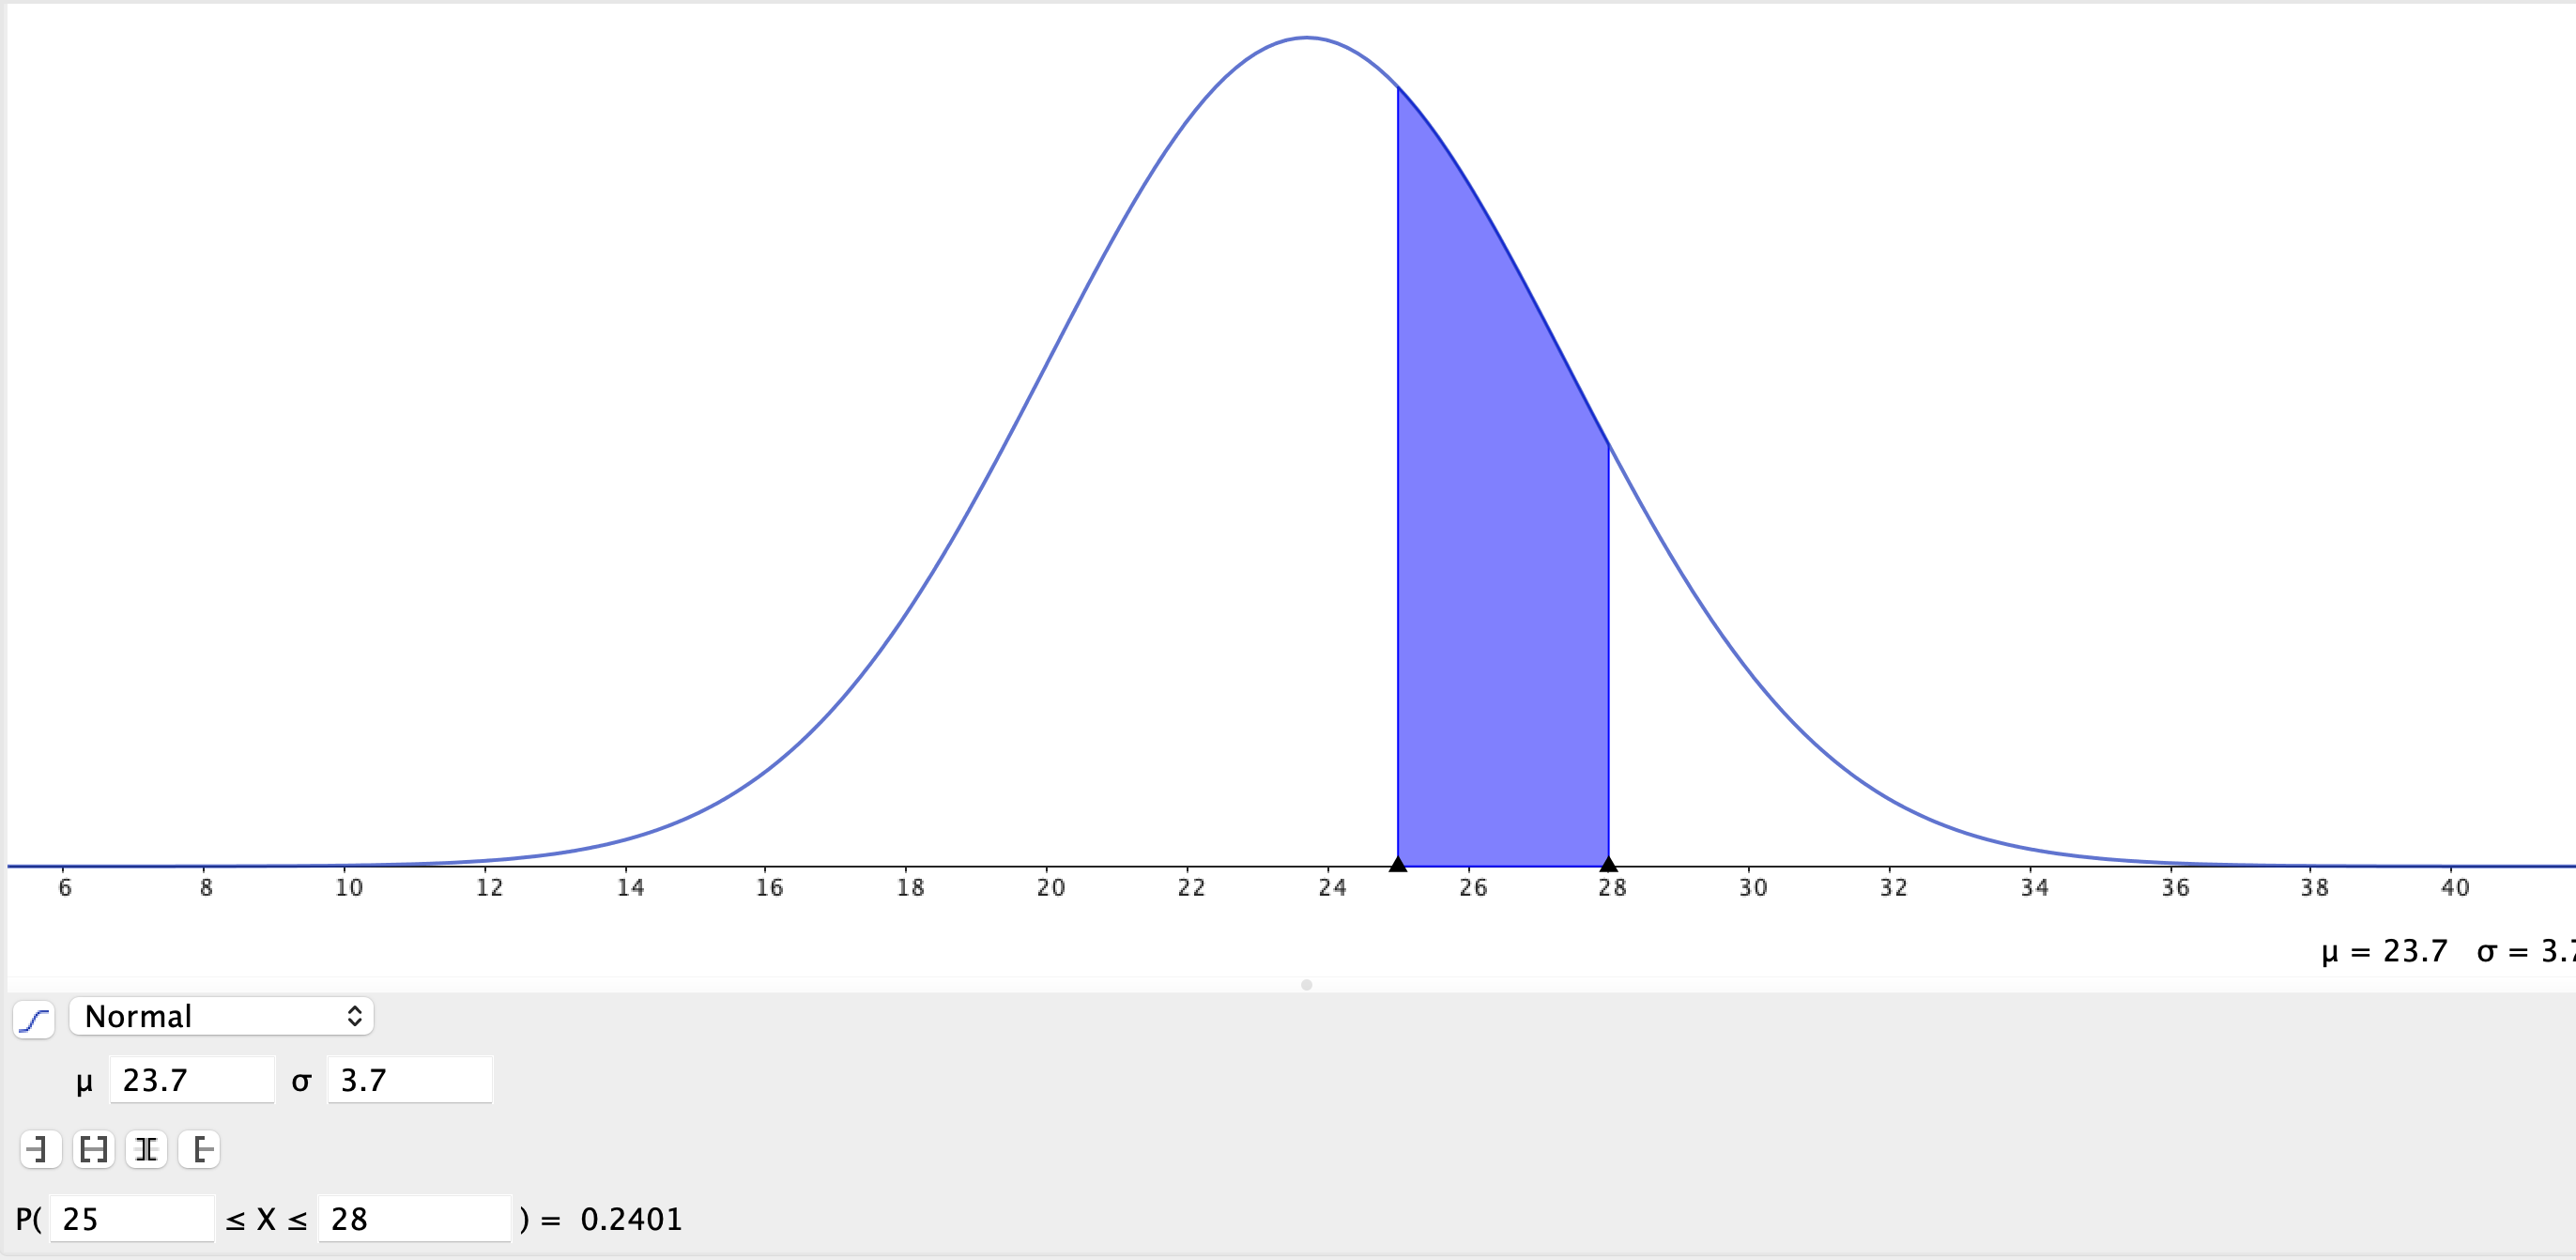
\includegraphics[width=\textwidth]{CASBMI.png}
\end{center}
\caption{Sandsynligheden bestemt med CAS}
\label{fig:CASBMI}
\end{figure}

Sandsynligheden for, at et individs BMI er mellem $25 \;\unit{kg/m^2} $ og $28 \;\unit{kg/m^2} $ er altså $0,2401$.\\[1ex]
\textbf{c.}
De exceptionelle udfald for individernes BMI er blot udfaldende, der er over tre spredninger fra middelværdien.
\begin{equation*}
\begin{split}
  ]-\infty ; \mu - 3 \sigma [ \,\cup\, ]\mu +3 \sigma ; \infty [ &=\, ]-\infty ; 23,7 - 3 \cdot 3,7 [ \, \cup \, ] 23,7 +3 \cdot 3,7 ; \infty [ \\
  &=\,]-\infty ;12,6[ \,\cup\, ]34,8;\infty [
\end{split}
\end{equation*}
De exceptionelle udfald for individernes BMI målt i $\unit{kg/m^2}$ er altså $\,]-\infty ;12,6[ \,\cup\, ]34,8;\infty [$. 

\begin{question}{Normalfordelt stokastisk variabel}{}
  En normalfordelt stokastisk variabel $X$ er givet ved $X \sim N(5,1)$. 
\end{question}
\sol \\
\textbf{a.}
Grafen for fordelingsfunktionen hørende til $X$ ses i \cref{fig:fordeling}. 
\begin{figure}[H]
\begin{center}
  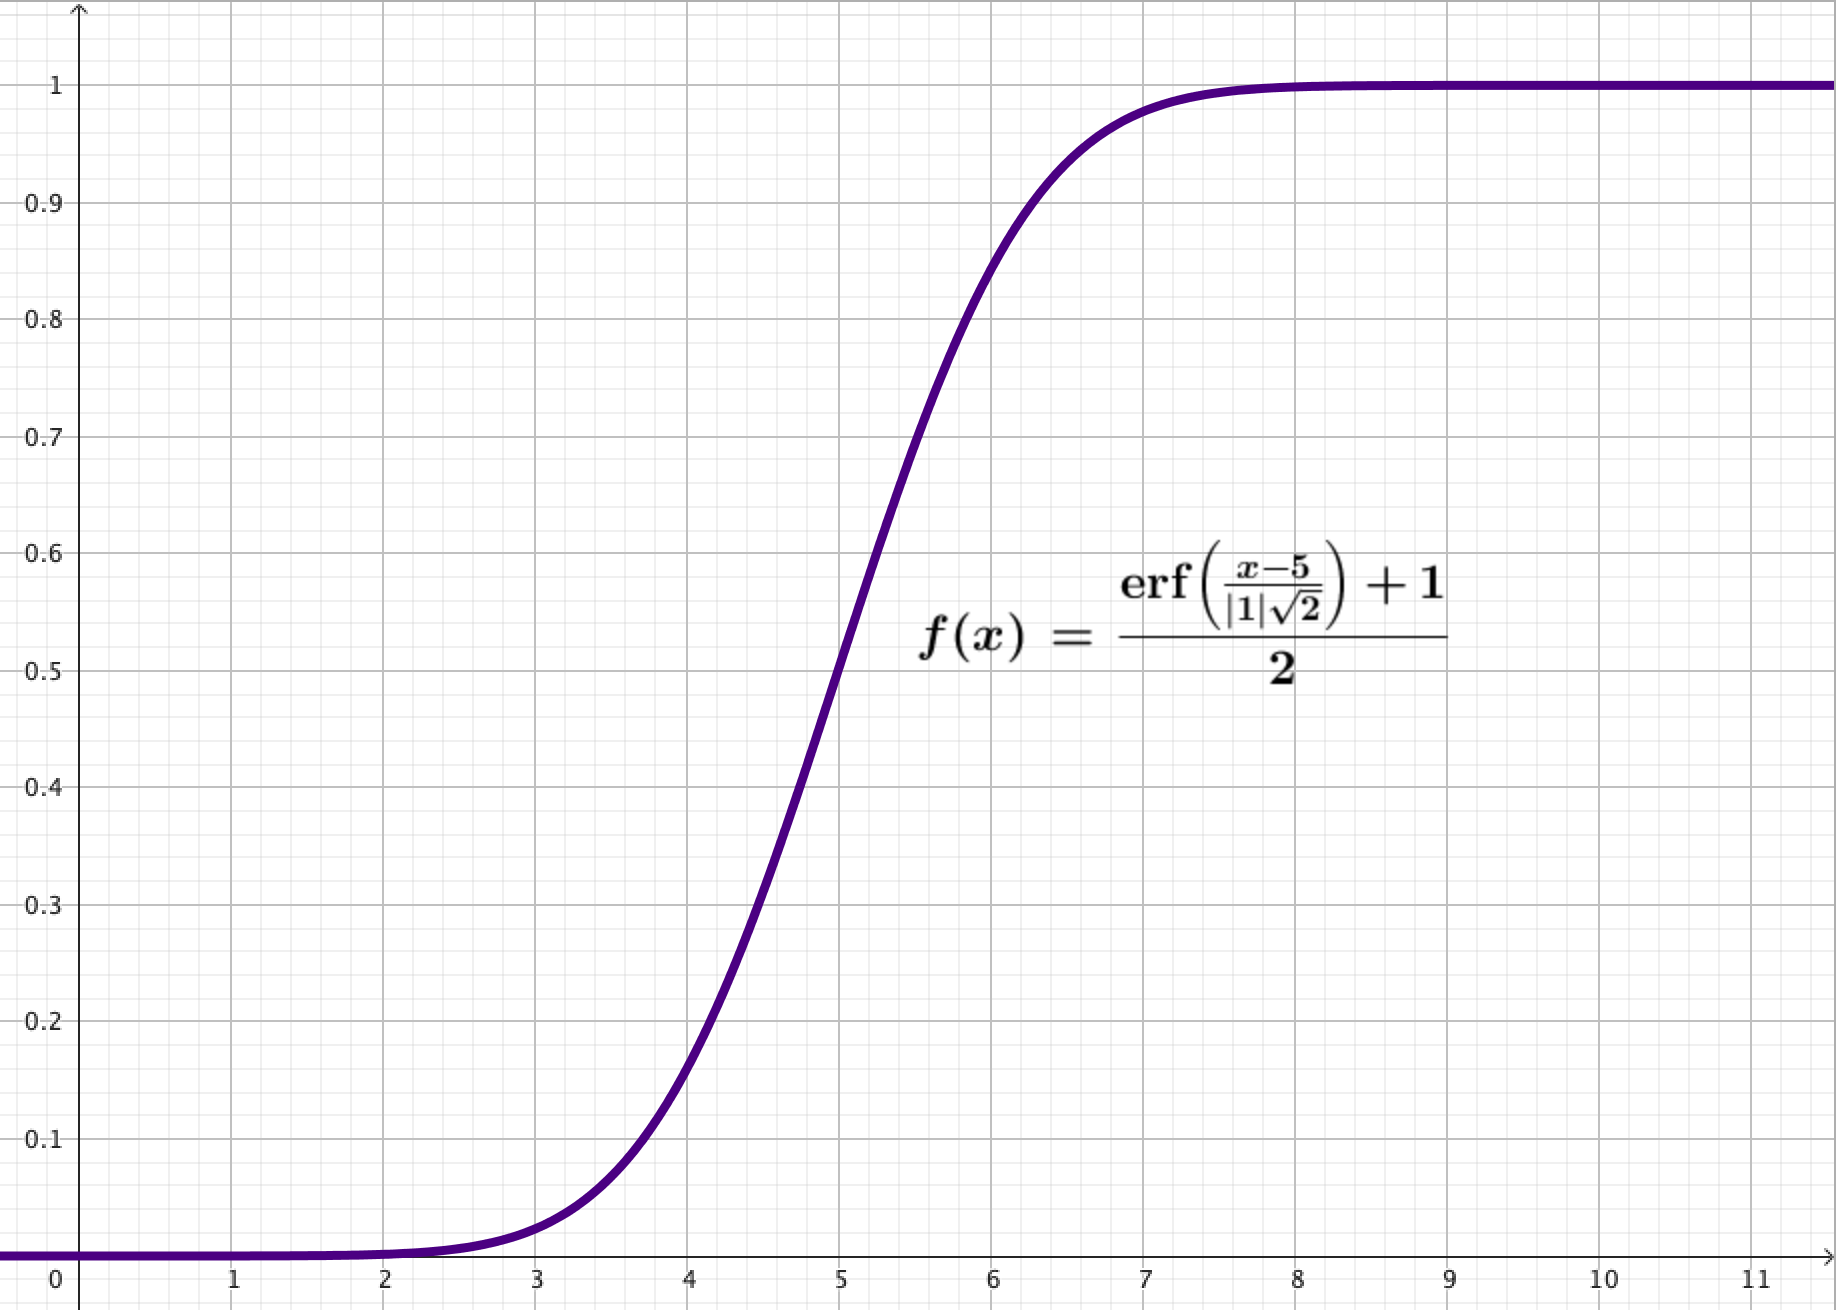
\includegraphics[width=0.8\textwidth]{fordeling.png}
\end{center}
\caption{Grafen for fordelingsfunktionen hørende til $X$}
\label{fig:fordeling}
\end{figure}
\noindent \textbf{b.}
For at bestemme $k$ benytter vi fraktilfunktionen.
Lad $F$ betegne fordelingsfunktionen hørende til $X$ (bemærk $F$ er injektiv), så gælder
\begin{equation*}
\begin{split}
  P(X \leq k) =0,4 &\iff F(k) =0,4 \\
  &\iff k=F ^{-1}(0,4).
\end{split}
\end{equation*}
Vi beregner $F ^{-1}(0,4)$ med CAS, hvilket ses i \cref{fig:fraktil04}.
\begin{equation*}
\begin{split}
  k&=F ^{-1}(0,4)\\
  &\approx 4,7467
\end{split}
\end{equation*}
Når $P(X \leq k) =0,4$, så er $k$ altså $4,7467$. 
\begin{figure}[H]
\begin{center}
  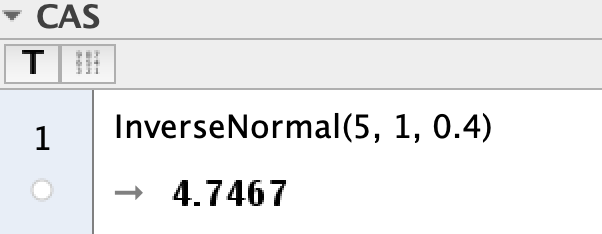
\includegraphics[width=0.7\textwidth]{fraktil04}
\end{center}
  \caption{$F ^{-1}(0,4)$ udregnet med CAS }
\label{fig:fraktil04}
\end{figure}

\begin{question}{Normalfordelte tulipanstilke}{}
  På et gartneri udvælger man på tilfældig måde 200 fuldt udvoksede tulipaner af en bestemt art.
  Man måler længden af deres stilke, og udvælger en tilfældig tulipan af denne art.
\end{question}
\sol \\
\textbf{a.}
For at redegøre for, at længden af tulipanstilkene med god tilnærmelse kan beskrives ved en normalfordelt stokastisk variabel $X$, laves et fraktilplot, hvilket ses i \cref{fig:fraktilplot}.

Det ses, at punkterne med god tilnærmelse ligger på linjen i fraktilplottet, hvilket vil sige, at længderne af tulipanstilkene med god tilnærmelse kan beskrives ved en normalfordelt stokastisk variabel $X$.
\begin{figure}[H]
\begin{center}
  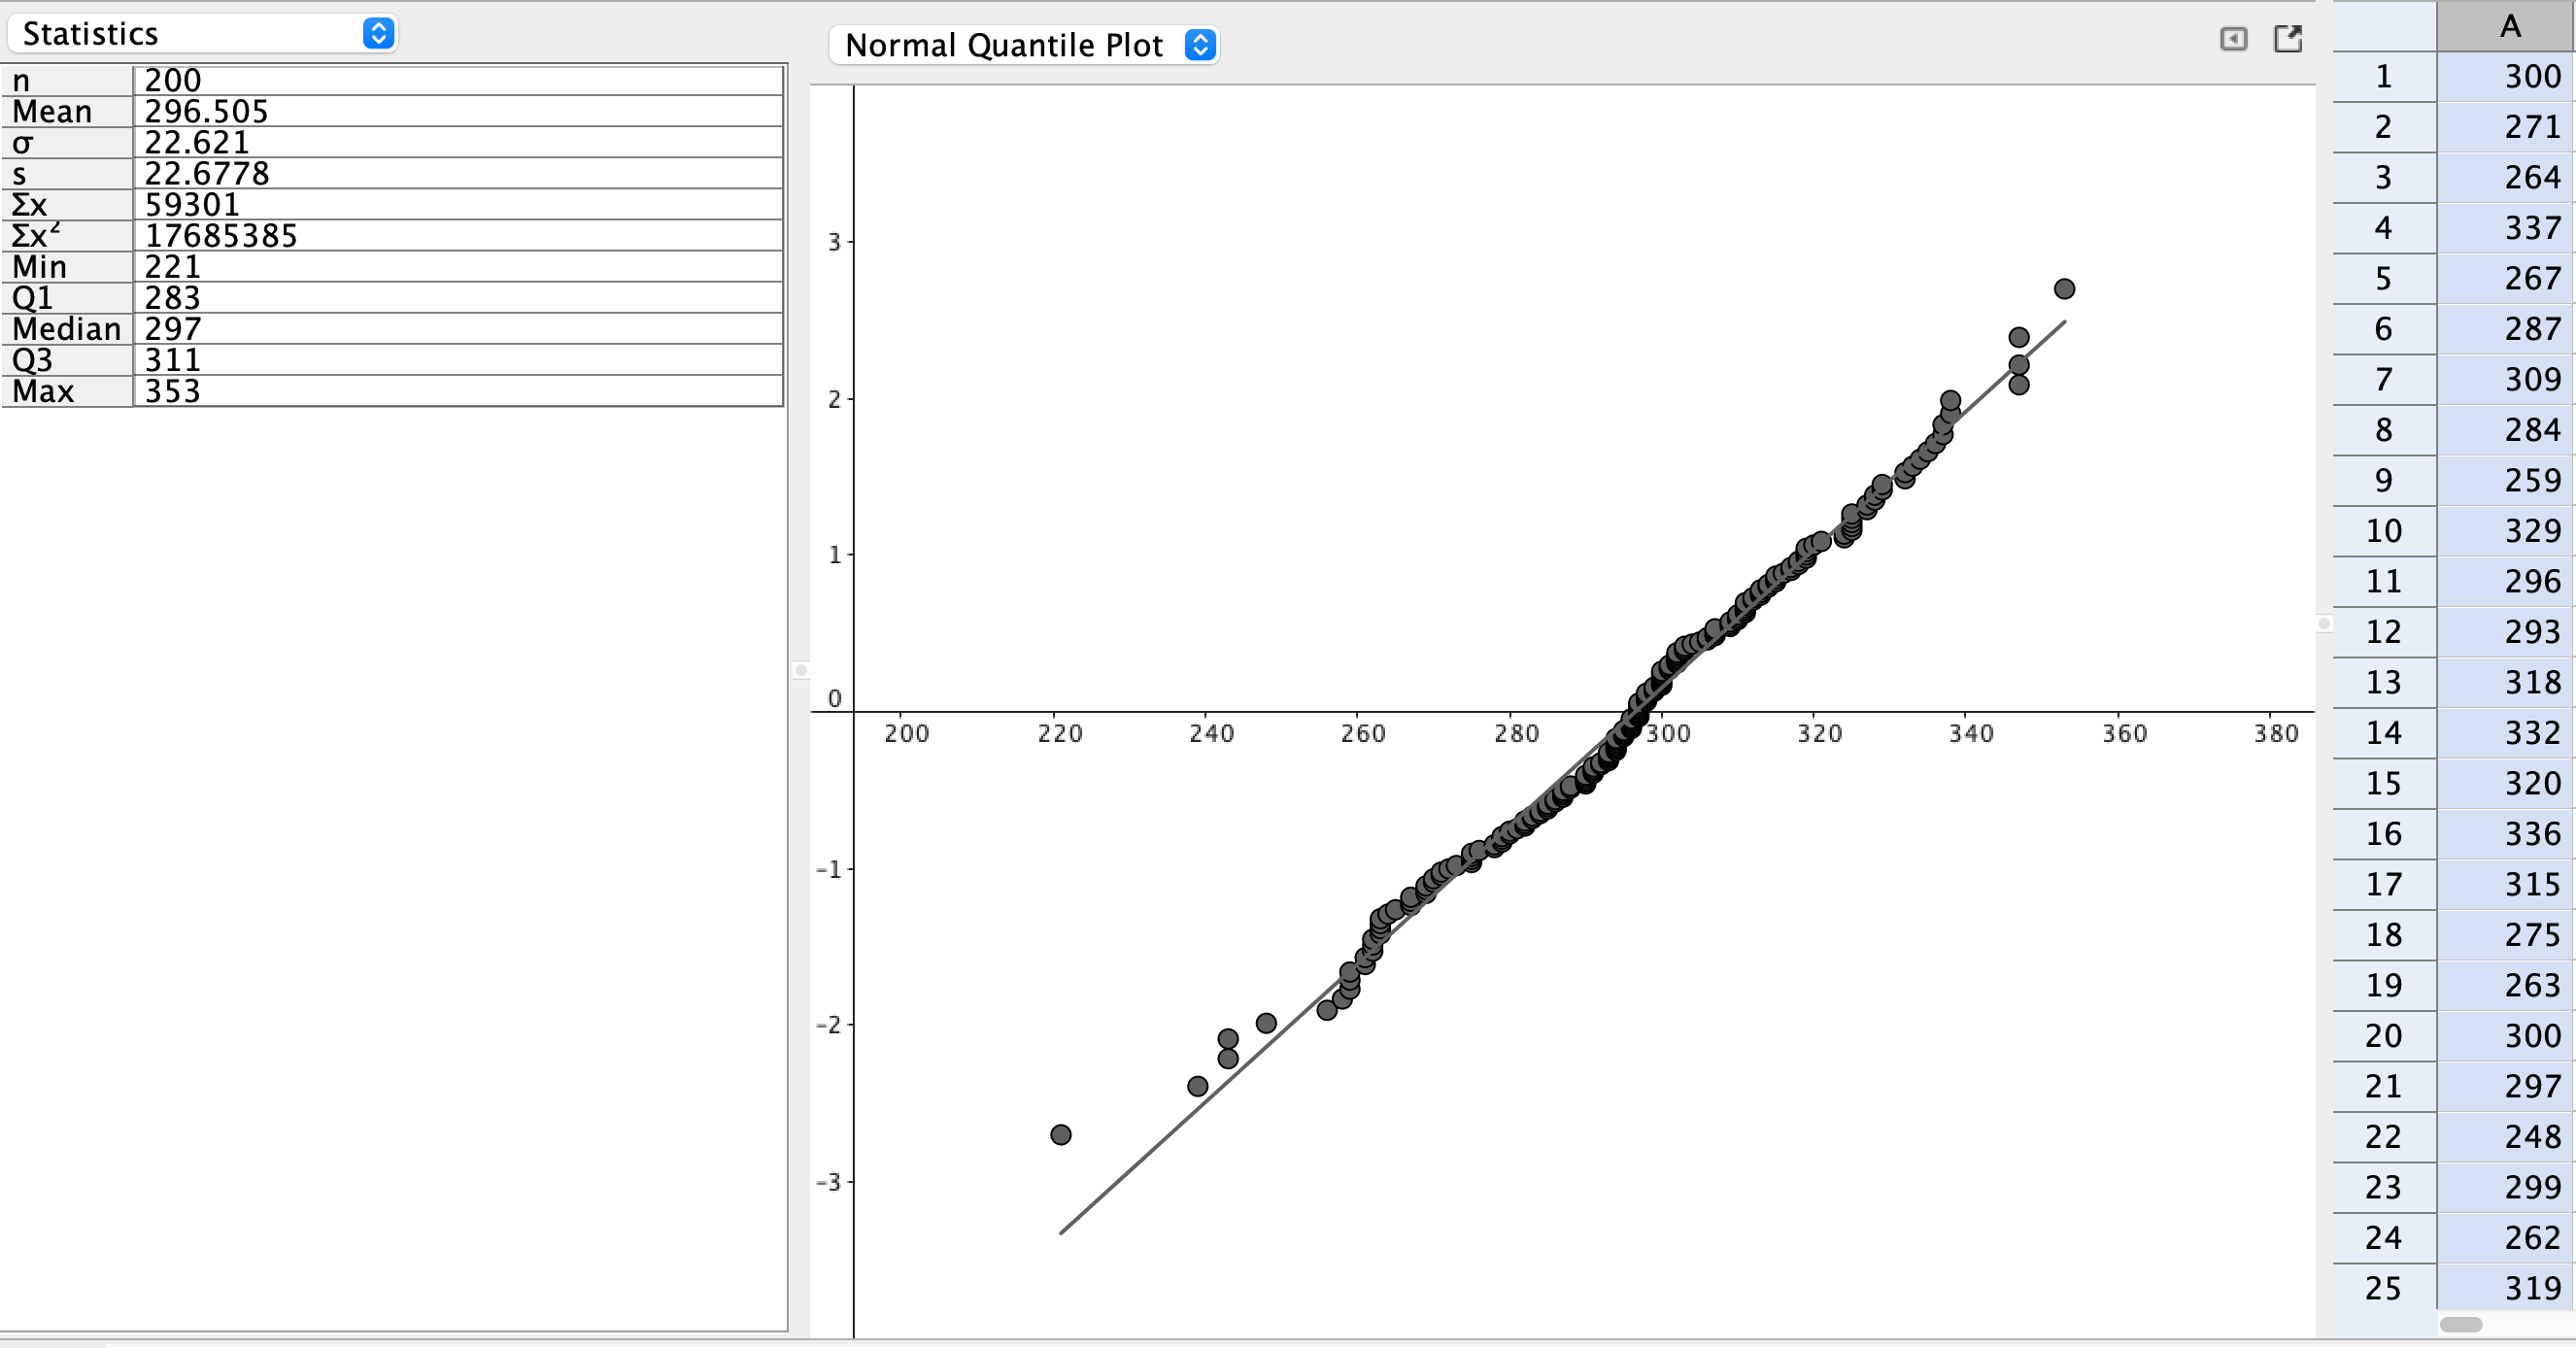
\includegraphics[width=\textwidth]{fraktilplot.png}
\end{center}
\caption{Fraktilplot lavet i GeoGebra}
\label{fig:fraktilplot}
\end{figure}
\noindent \textbf{b.}
Fra \cref{fig:fraktilplot} har vi, at $X$ har middelværdien (i mm) $\mu =296,505$ og spredningen (i mm) $\sigma = 22,6778$.\\[1ex]
\textbf{c.}
Vi bestemmer sandsynligheden $P(270 \leq X \leq 330)$ med CAS, hvilket ses i \cref{fig:CASstilke}. 
\begin{equation*}
\begin{split}
  P(270 \leq X \leq 330)&=P(X \leq 330)-P(X \leq 270)\\
  &\approx 0,8089 \\
  &=80,89 \%
\end{split}
\end{equation*}
Sandsynligheden for, at længden af stilken er mellem 270 mm og 330 mm er altså $80,89 \%$.
\begin{figure}[H]
\begin{center}
  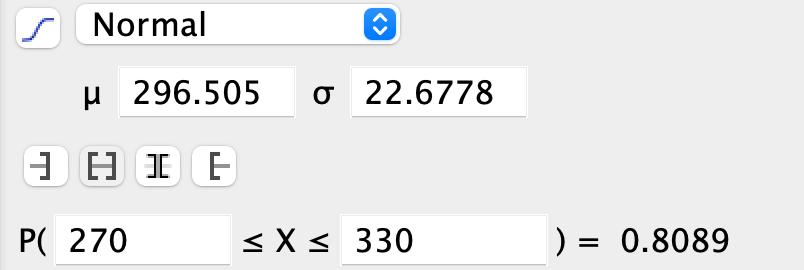
\includegraphics[width=0.8\textwidth]{CASstilke.png}
\end{center}
\caption{Sandsynligheden udregnet med CAS}
\label{fig:CASstilke}
\end{figure}

\begin{question}{Model for benzinforbrug i USA}{}
  Tabellen viser udviklingen i benzinforbruget (målt i mia. gallon) i USA i årene 1992-2004.
  I en model kan udvilklingen beskrives ved
  \[
  f(x)= ax + b,
  \] 
  hvor $f(x)$ er benzinforbruget i USA (målt i mia. gallon), og $x$ er altsl år efter 1992. 
  I 2019 var benzinforbruget i USA 142 mia. gallon.
\end{question}
\sol \\
\textbf{a.}
Vi bestemmer tallene $a$ og $b$ ved lineær regression på tabellens data, hvilket ses i \cref{fig:gallon}. 
Fra regressionen har vi, at
\[
a=2,1758 \text{ og } b=109,1758.
\] 
\begin{figure}[H]
\begin{center}
  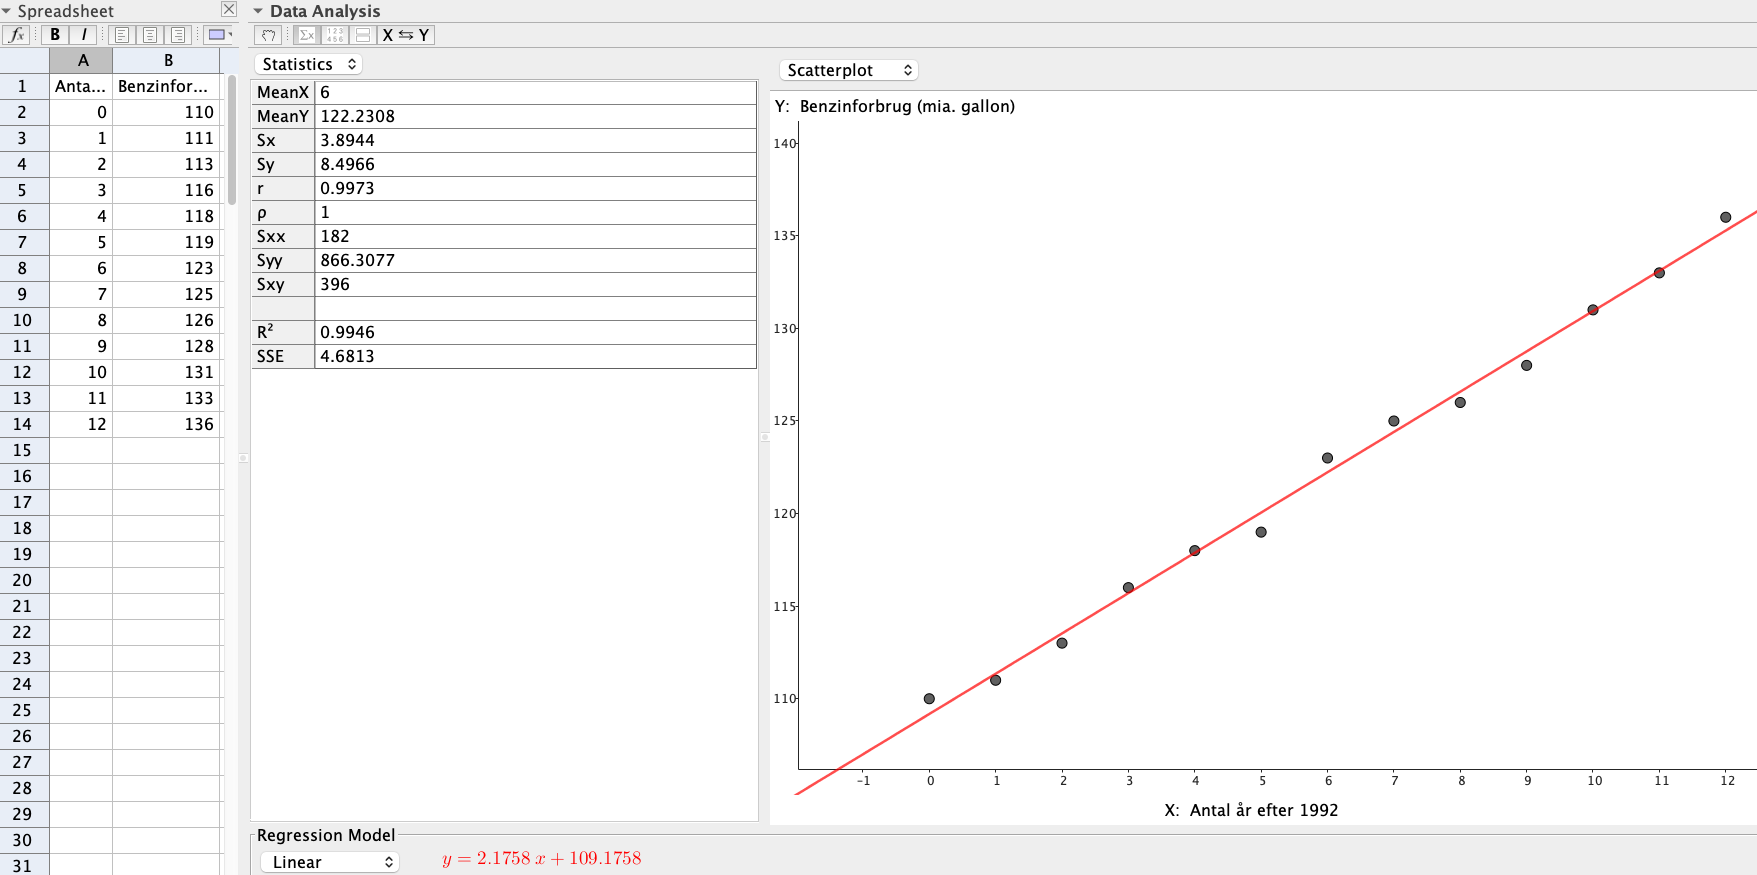
\includegraphics[width=\textwidth]{gallon.png}
\end{center}
\caption{Lineær regression på tabellens data}
\label{fig:gallon}
\end{figure}

\noindent \textbf{b.}
Et residualplot ses tegnet i \cref{fig:gallonresidual}.
Det ses, at punkterne ligger nogenlunde tilfældigt fordelt omkring linjen med forskriften $x=0$.
Altså passer modellen tilnærmelsesvist med udviklingen i perioden 1992-2004.
\begin{figure}[H]
\begin{center}
  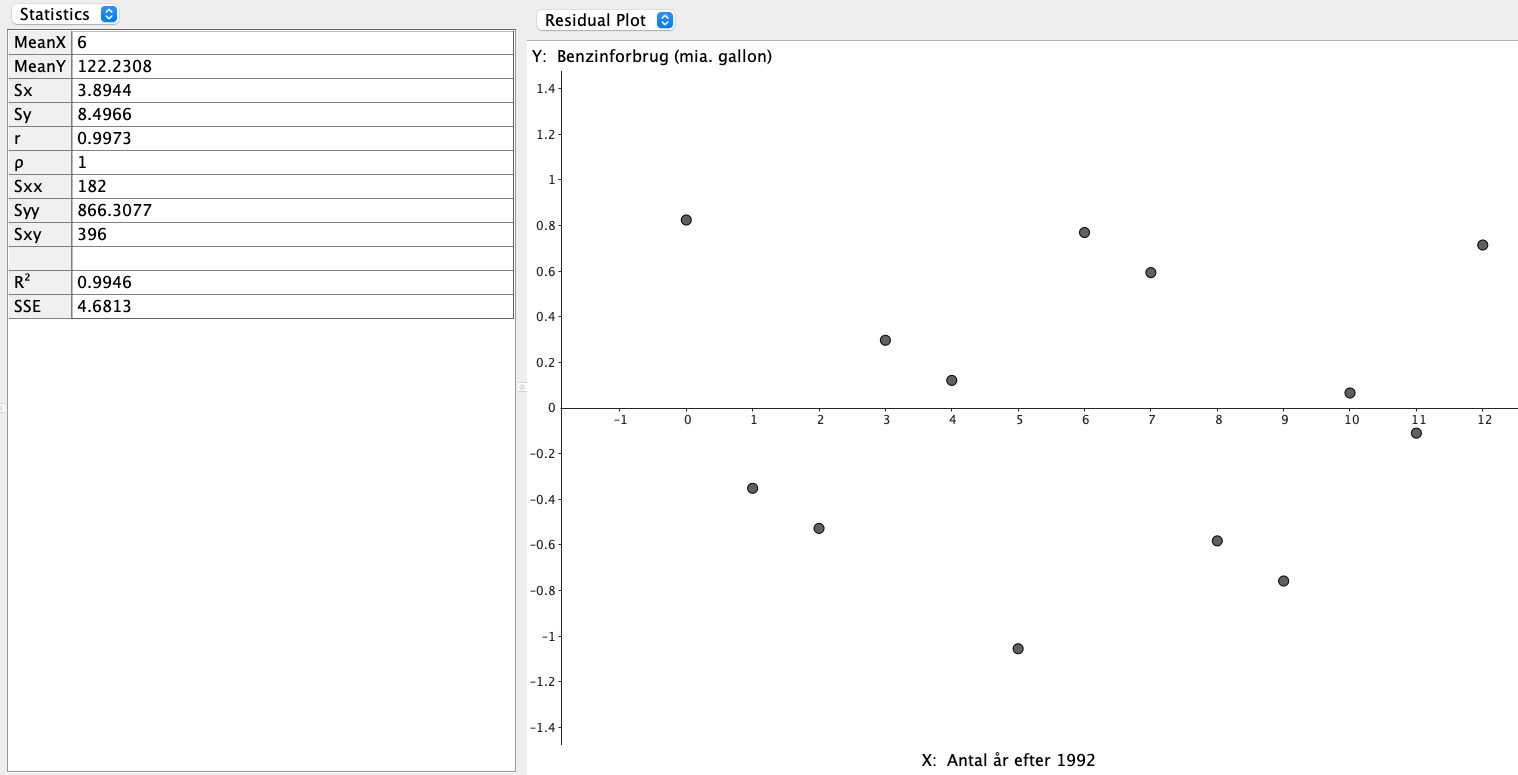
\includegraphics[width=0.7\textwidth]{gallonresidual.png}
\end{center}
\caption{Residualplot}
\label{fig:gallonresidual}
\end{figure}

\noindent \textbf{c.}
For at beregne $f(27)$, opskriver vi først en forskrift for $f$.
Fra regressionen havde vi, at 
\[
f(x)= 2,1758 \cdot x + 109,1758.
\] 
Vi beregner nu $f(27)$.
\begin{equation*}
\begin{split}
  f(27)&=2,1758 \cdot 27 + 109,1758\\
  &\approx 167,92.
\end{split}
\end{equation*}
Benizinforbruget i USA i 2019 (142 mia. gallon) var altså mindre end ifølge modellen (167,92 mia. gallon).

\begin{question}{Lineær model for blomsterdata}{}
 Tabellen viser en række målinger af sammenhørende værdier af nogle kronblades bredde og længde for en bestemt blomsterart.
 I en lineær regressionsmodel kan sammenhængen mellem bredden og længden af et kronblad beskrives ved
  \[
  f(x)= a \cdot x + b,
  \] 
  hvor $f(x)$ betegner længden af et kronblad (målt i cm) med bredden $x$ (målt i cm).
  En gruppe biologer formoder, at den lineære sammenhæng mellem længden og bredden af et kronblad er voksende.
\end{question}
\sol \\
\textbf{a.}
For at redegøre for, at residualerne i modellen med god tilnærmelse er normalfordelte, laver vi et fraktilplot med residualerne, hvilket ses i \cref{fig:resifraktil}.
Det ses, at punkterne med god tilnærmelse ligger på linjen i fraktilplottet.
Altså kan residualerne i modellen med god tilnærmelse siges at være normalfordelte.

\begin{figure}[H]
\begin{center}
  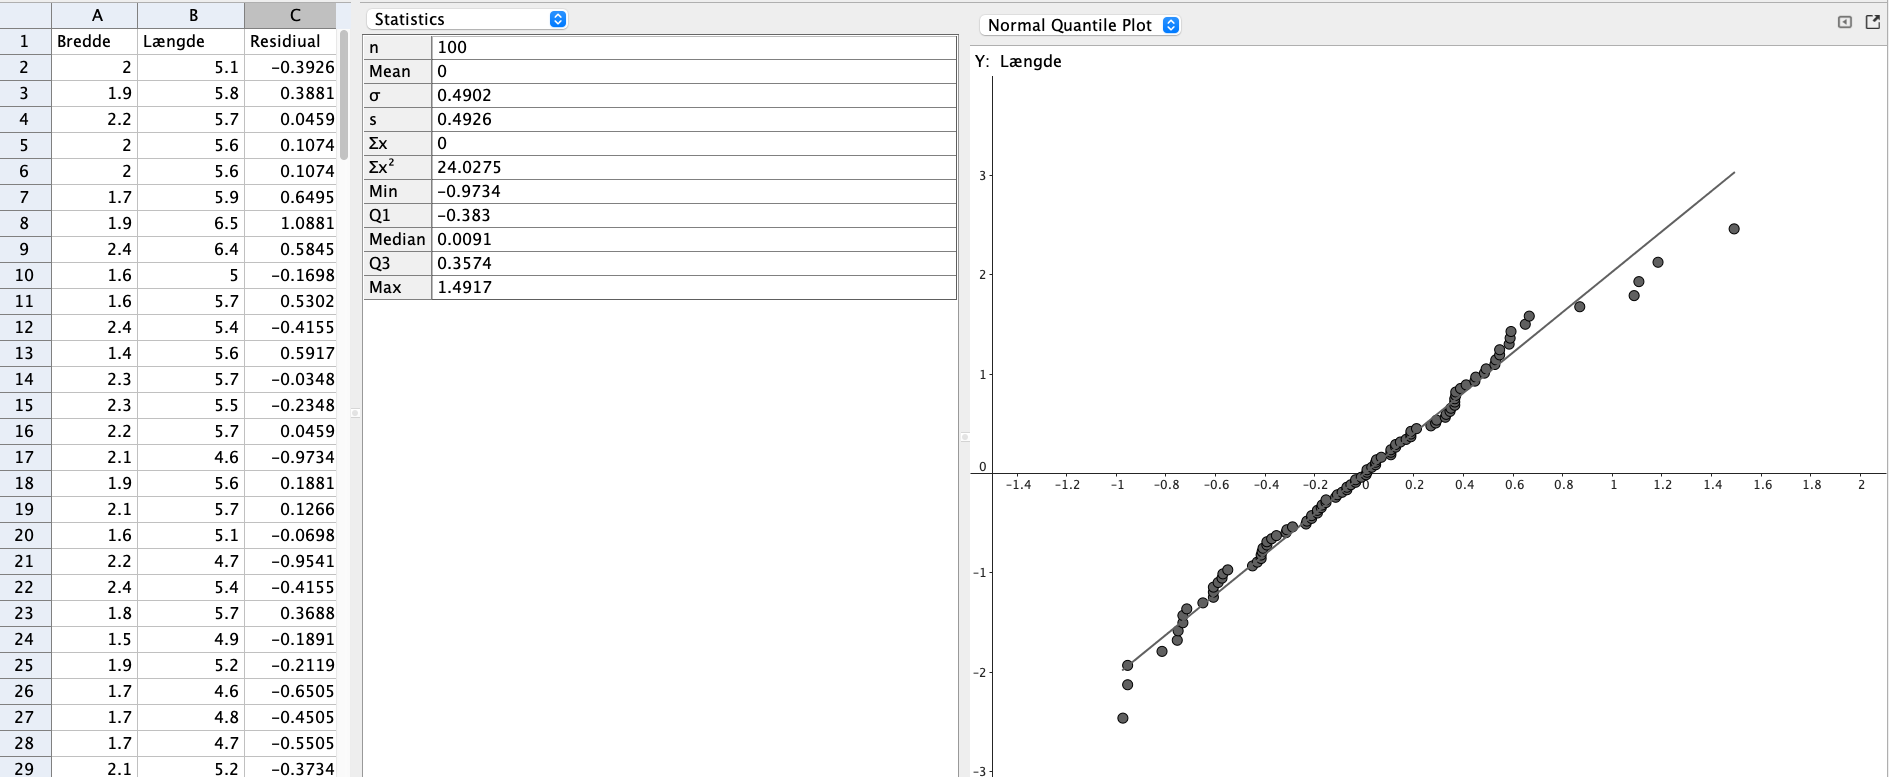
\includegraphics[width=\textwidth]{resifraktil.png}
\end{center}
\caption{Fraktilplot for residualerne}
\label{fig:resifraktil}
\end{figure}

\noindent\textbf{b.}
Et 95\% konfidensinterval for hældningskoeffienten i modellen findes med GeoGebra, hvilket ses i \cref{fig:konfidens}.
Fra GeoGebra har vi, at et 95 \% konfidensinterval for hældningskoefficienten i modellen er $[0,4925;1,1219]$.
Siden der gælder, at 
\[
[0,4925 ; 1,1219] \subset \mathbb{R}^+,
\] 
så er den lineære sammenhæng mellem længden og bredden af et kronblad voksende.
Altså er biologernes formodning troværdig.

\begin{figure}[H]
\begin{center}
  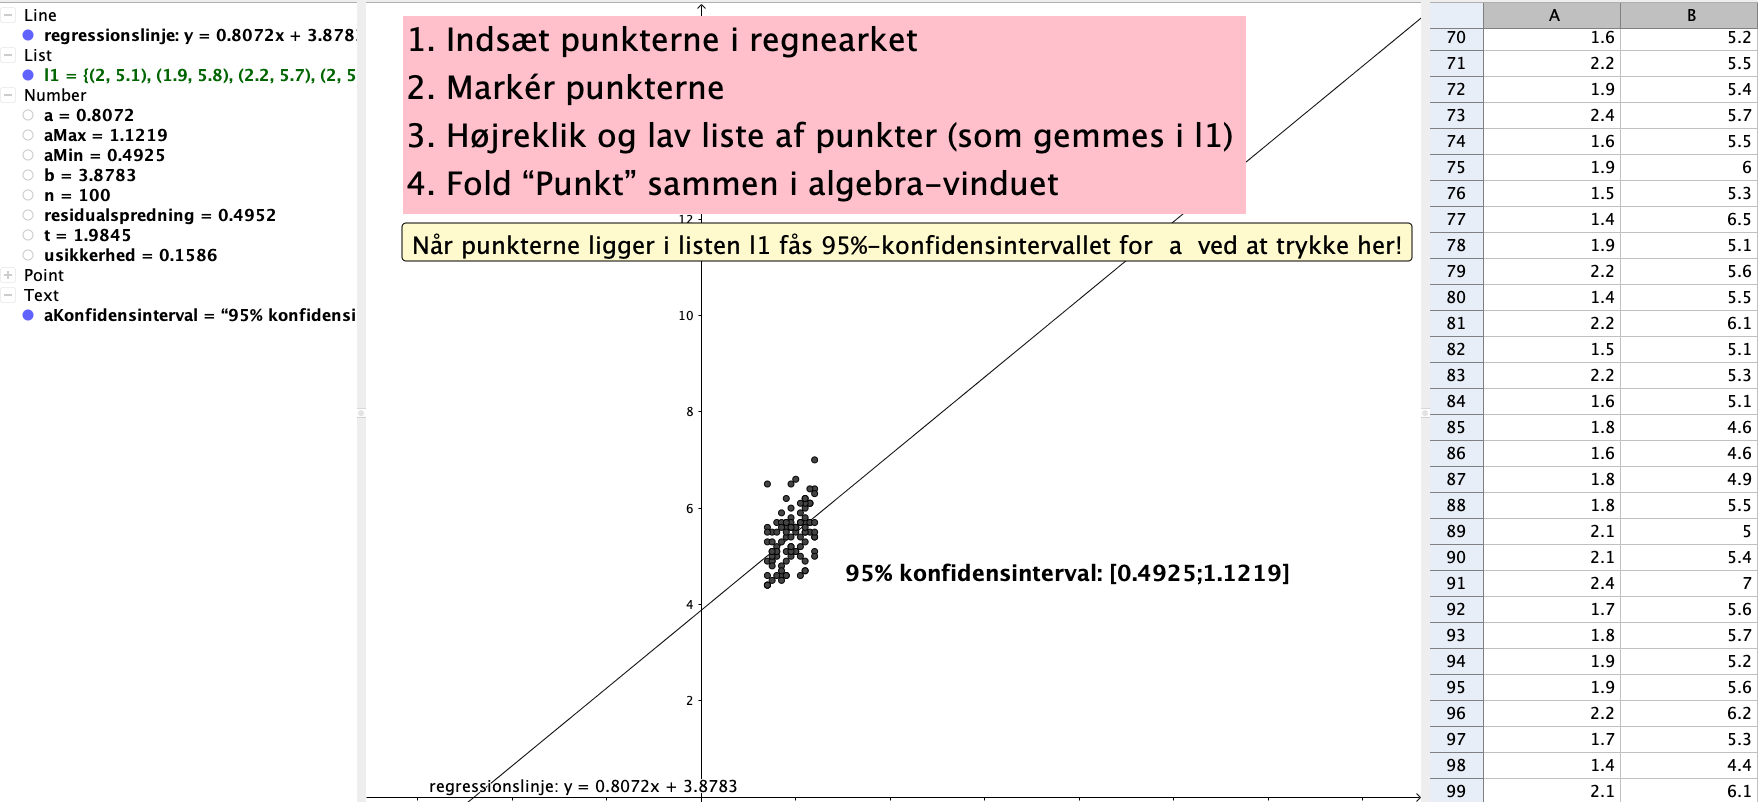
\includegraphics[width=0.9\textwidth]{konfidens.png}
\end{center}
\caption{95 \% konfidensinterval for hældningskoefficiente}
\label{fig:konfidens}
\end{figure}

\begin{question}{Lineær model for hjernevægt}{}
  Tabellen viser sammenhørende værdier for rumfanget af en mands hovede og vægten af hans hjerne.
  I en model kan sammenhængen beskrives ved
  \[
  f(x)= a \cdot x + b,
  \] 
  hvor $f(x)$ betegner vægt (målt i gram), og $x$ betegner rumfang (målt i $\unit{cm^3}$).
\end{question}
\sol \\
\textbf{a.}
For at bestemme tallene $a$ og $b$, laver vi en lineær regression på tabellens data, hvilket ses i \cref{fig:rumfangregression}.
Fra regressionen har vi, at
\[
a=0,1985 \text{ og } b=597,8387.
\] 
\begin{figure}[H]
\begin{center}
  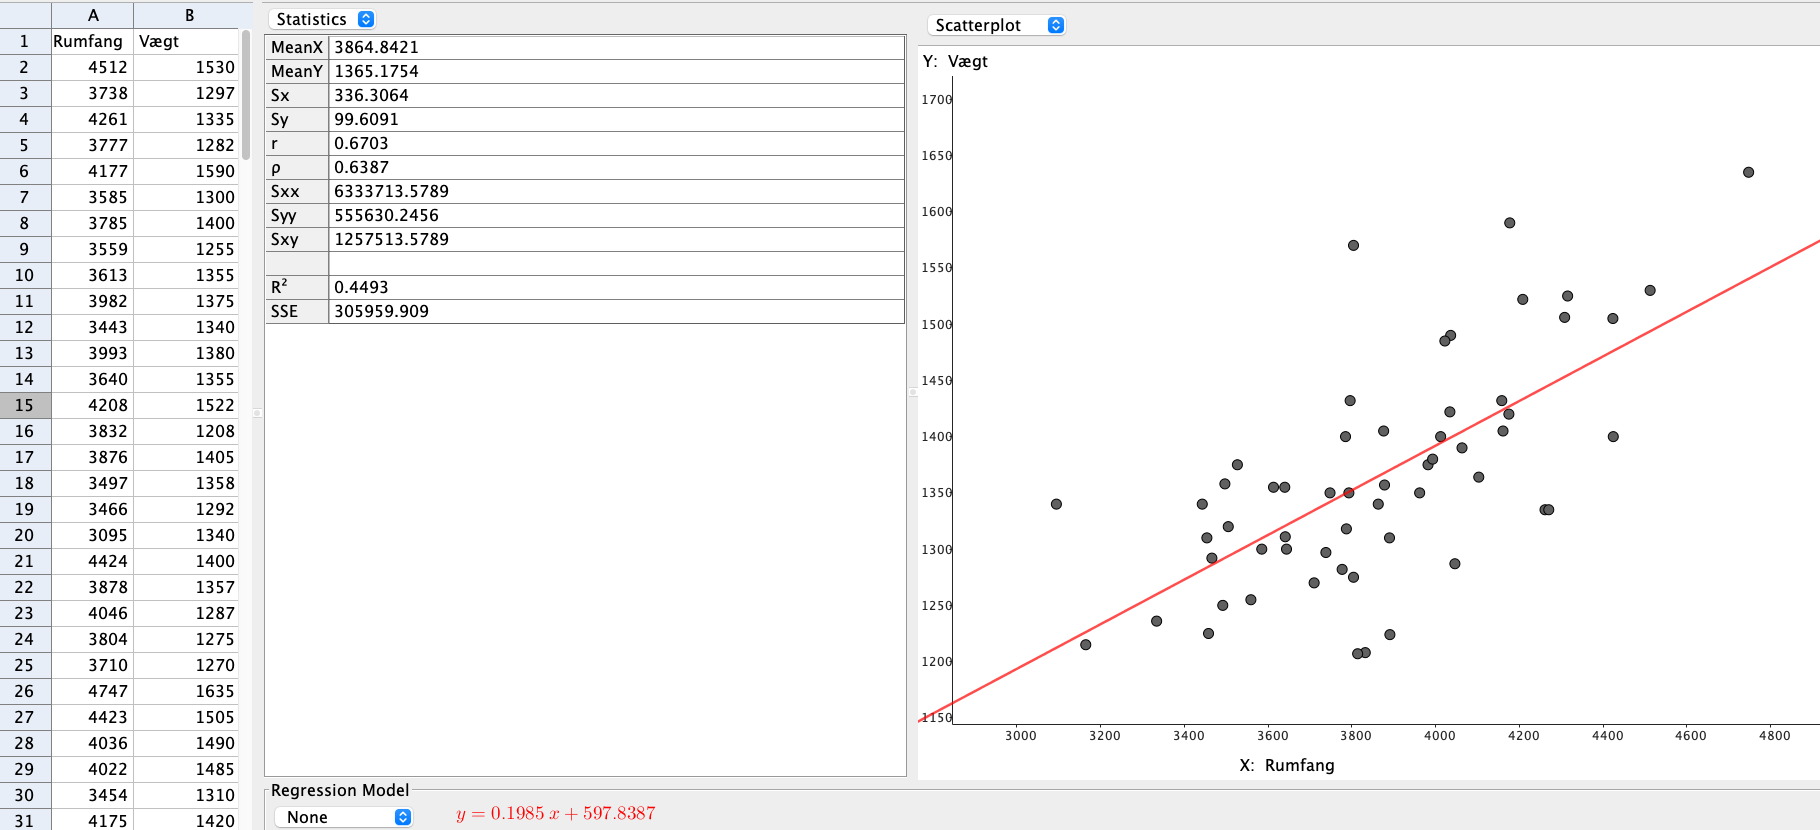
\includegraphics[width=0.8\textwidth]{rumfangregression.png}
\end{center}
\caption{Lineær regression på tabellens data}
\label{fig:rumfangregression}
\end{figure}

\noindent \textbf{b.}
Givet et endeligt antal residualer $r_1, r_2, \ldots, r_n$ er residualspredningen givet ved
\[
s=\sqrt{\frac{r_1^2 + r_2^2 + \cdots + r_n^2}{n-2}}.
\] 
Denne beregner vi med GeoGebra, hvilket ses i \cref{fig:residualspredning}.
Vi har beregnet residualspredningen til at være $74,5849$.
\begin{figure}[H]
\begin{center}
  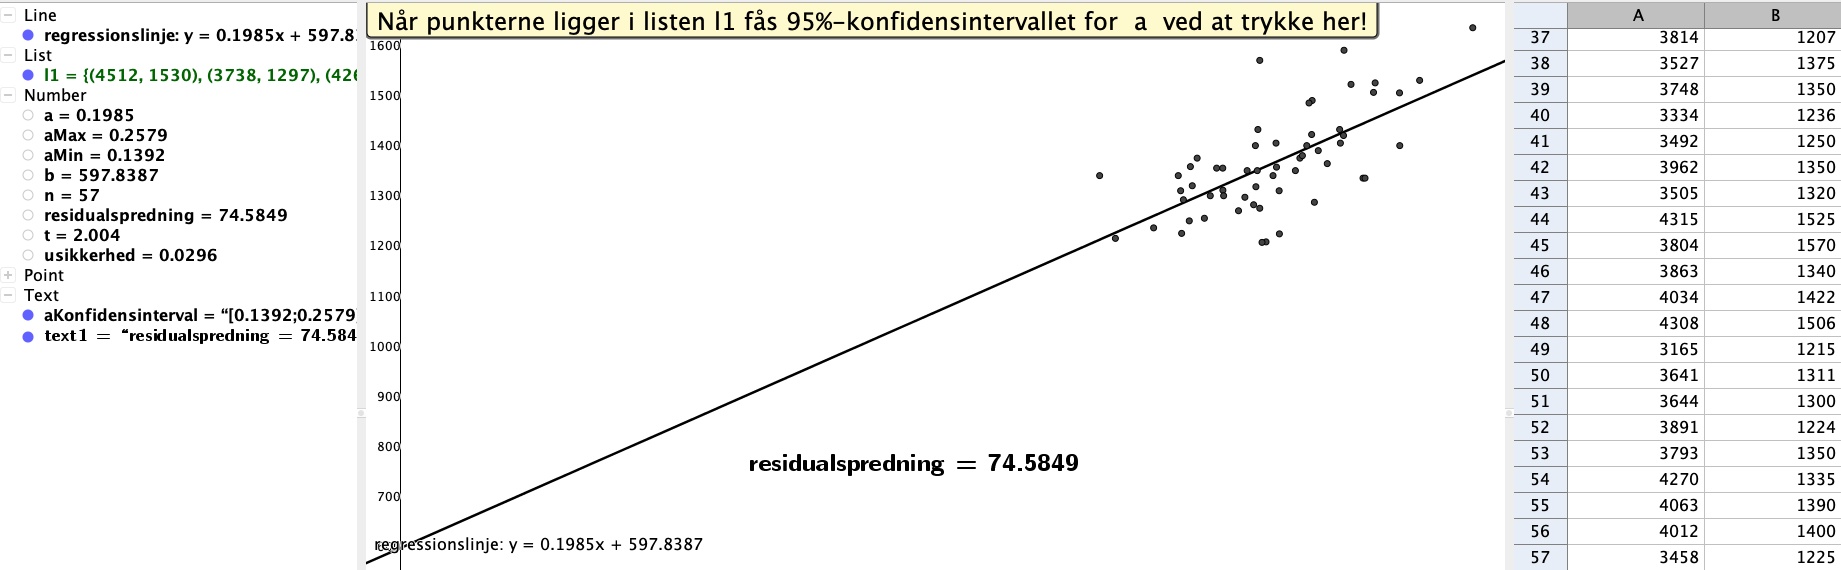
\includegraphics[width=0.8\textwidth]{residualspredning.png}
\end{center}
\caption{Residualspredningen}
\label{fig:residualspredning}
\end{figure}


\end{document}
